\documentclass{article}
\usepackage{tikz}
\usetikzlibrary{intersections,angles,quotes}

\setlength{\parindent}{0pt}

\begin{document}
Friccción: $F = \mu \vec{N}$ donde $\mu$ es un constante y $\vec N$ es la normal de una fuerza.



Tensión: Fuerza desde ambos extremos de una cuerda hacia adentro de la misma. 

\begin{center}
  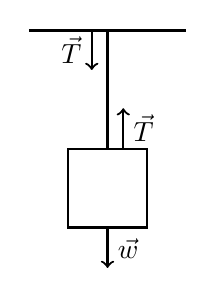
\begin{tikzpicture}[thick]
    \node[rectangle, minimum width=1cm, minimum height=1cm, draw]
      (rect) at (0,0)
      {};
    \draw
      (-1,2) -- (1,2)
      (rect) -- (0,2)
      (0,2 -| -0.2,0) edge[->] node[left] {$\vec T$} ++(0,-0.5)
      (rect.north -| 0.2,0) edge[->] node[right] {$\vec T$} ++(0,0.5)
      (rect.south) edge[->] node[right] {$\vec w$} ++(0,-0.5) 
      ;
  \end{tikzpicture}
\end{center}

Plano incinado\\
$P_x$ = $P \sin{\alpha}$\\
$P_y$ = $P \cos{\alpha}$

\begin{center}
  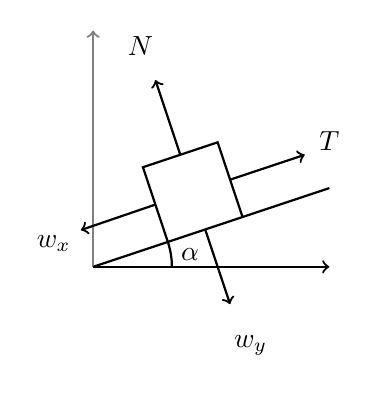
\begin{tikzpicture}[thick]
    \draw
      (0,0) edge[->,draw=gray] (0,3)
      (0,0) edge[->] (3,0)
      (0,0) -- (3,1)
      (1,0) arc  (0:18.44:1) node[midway,right]  {$\alpha$} coordinate (a)
      (a) -- ++(18.44:1) coordinate[midway] (d) {} -- ++(108.44:1) coordinate[midway] (b) -- ++(198.44:1) coordinate[midway] (e) -- ++(288.44:1) coordinate[midway] (c)
      (b) edge[->] ++(18.44:1) 
      (c) edge[->] ++ (198.88:1)
      (d) edge[->] ++(288.44:1)
      (e) edge[->] ++(108.44:1)
      (3,1.6) node {$T$}
      (-0.5,0.3) node {$w_x$}
      (2,-1) node {$w_y$}
      (0.6,2.8) node {$N$}
      ;
  \end{tikzpicture}
\end{center}

\[
  \vec{F} = m\vec{a}
\]
\[
  \vec{F}_{T} = w + N + T + f?
\]

\section*{Movimiento circular uniforme}

\begin{center}
  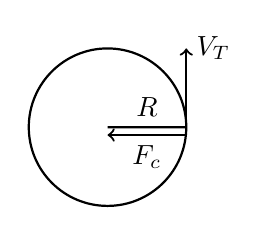
\begin{tikzpicture}[thick]
    \draw
      (0,0) circle (1)
      (0,0) -- (1,0) node[midway,above] {$R$}
      (1,-0.1) edge[->] (0,-0.1) node[midway,below=3pt] {$F_c$}
      (1,0) edge[->] (1,1) 
      (1,1) node[right] {$V_T$}
      ;

  \end{tikzpicture}
\end{center}

$a = \frac{v^2}{R}$: Aceleración centrípeta 

$F_c = ma$: Fuerza centrípeta

\section* a

\pgfdeclarelayer{background layer}
\pgfdeclarelayer{foreground layer}
\pgfsetlayers{background layer,main,foreground layer}
\begin{tikzpicture}[thick]
  \coordinate (A) at (0,0);
  \coordinate (B) at (5,0);
  \coordinate (C) at (0,5);
  \draw (B) -- (A);
  \path[name path = vert] (A)--(C);
  \path[name path = hvert] (2.5,0)--++(0,5);

%For intersections
  \path[name path = angled] (B) -- +(160:6cm);
  \path [name intersections={of=vert and angled, by={a}}];
  \path [name intersections={of=hvert and angled, by={b}}];

  \draw (B) -- (a);
  \begin{pgfonlayer}{background layer}
    \node[anchor=south,rotate=-20,inner sep=0pt] (car) at (b) {\includegraphics[height=2cm]{car.png}}; 
  \end{pgfonlayer}

  \coordinate (c) at (3,1.7); 
  \draw[thick,->] (c) -> ++(0,-2) node[below] {w};
  \draw[thick,->] (c) -> ++(70:2) node[above] {N};
  \draw[thick,->] (c) -> ++(1,0) node[right] {$F_n = \frac{m~ v^2}{\rho}$}
    ;
  \pic["$\alpha$", draw,angle radius=1.3cm] {angle = a--B--A};
\end{tikzpicture}

\end{document}
